

\documentclass[18pt]{beamer}

\usepackage[utf8]{inputenc}
\usepackage{graphicx}
\graphicspath{ {images/} }

\usepackage{templates/beamerthemekit}
%\usepackage{templates/beamerthemekitwide}

%% TITLE PICTURE

% if a custom picture is to be used on the title page, copy it into the 'logos'
% directory, in the line below, replace 'mypicture' with the 
% filename (without extension) and uncomment the following line
% (picture proportions: 63 : 20 for standard, 169 : 40 for wide
% *.eps format if you use latex+dvips+ps2pdf, 
% *.jpg/*.png/*.pdf if you use pdflatex)

%\titleimage{Folientitelbild_wide}

%% TITLE LOGO

% for a custom logo on the front page, copy your file into the 'logos'
% directory, insert the filename in the line below and uncomment it

%\titlelogo{infofak}

% (*.eps format if you use latex+dvips+ps2pdf,
% *.jpg/*.png/*.pdf if you use pdflatex)



% the presentation starts here

\title[Flexible User-Friendly Trip Planning
Queries]{Bachelor's Thesis \\ Flexible User-Friendly Trip Planning Queries}
\subtitle{Adviser: Saeed Taghizadeh}
\author{Violina Zhekova}

\institute{IPD B{\"o}hm}


\begin{document}
	
% change the following line to "ngerman" for German style date and logos
\selectlanguage{english}

%title page
\begin{frame}
	\titlepage
\end{frame}

%table of contents
\begin{frame}{Outline}
	\tableofcontents
\end{frame}


\section{Motivation}
	\begin{frame}{Motivation}
	
		\begin{itemize}
			\item Sequenced Route Queries (SRQ) - finding routes passing through multiple Points of Interest (PoIs)
			\item Advances in Location Based Services (LBS)
			\item Geographic Information System (GIS) applications (e.g. logistics and supply chain management) \newline
		\end{itemize}
		
		\begin{figure}[h]
			
\includegraphics[scale=0.2]{Motivation.jpg}
		\end{figure}
	
	\end{frame}

\section{Related Work}
	\begin{frame}{Related work}
	
		\begin{itemize}
			\item Trip Planning Queries (TPQ)
			\item Optimal Sequenced Route (OSR) Query
			\item Skylyne concept 
			\item Considering multiple factors of a route – rating, distance and category weights
			\item SRQ issued by users moving along a route
			\newline
		\end{itemize}
	
	\end{frame}

\section{Problem Definition}
	\begin{frame}{Problem definition}
	
		\begin{itemize}
			\item
		\end{itemize}
	
	\end{frame}

\section{Introducing the Operators}

	\subsection{Equality}
		\begin{frame}{Equality}
			
			\begin{itemize}
				\item
			\end{itemize}
			
		\end{frame}
					
	\subsection{Inequality}
		\begin{frame}{Inequality}
		
			\begin{itemize}
				\item
			\end{itemize}
		
		\end{frame}
	
	\subsection{Or}
		\begin{frame}{Or}
		
			\begin{itemize}
				\item
			\end{itemize}
		
		\end{frame}
	
	\subsection{Order}
		\begin{frame}{Order}
		
			\begin{itemize}
				\item
			\end{itemize}
		
		\end{frame}
	
\section{Evaluating the operators}

	\subsection{Equality}
		\begin{frame}{Equality}
		
			\begin{itemize}
				\item
			\end{itemize}
		
		\end{frame}
	
	\subsection{Inequality}
		\begin{frame}{Inequality}
		
			\begin{itemize}
			\item
			\end{itemize}
		
		\end{frame}
	
	\subsection{Or}
		\begin{frame}{Or}
		
			\begin{itemize}
			\item
			\end{itemize}
		
		\end{frame}
	
	\subsection{Order}
		\begin{frame}{Order}
		
			\begin{itemize}
			\item
			\end{itemize}
		
		\end{frame}
	
\section{Conclusion}
	\begin{frame}{Problem definition}
	
		\begin{itemize}
			\item
		\end{itemize}
	
	\end{frame}

\section{Discussion and Future Work}
	\begin{frame}{Discussion and Future Work}
	
		\begin{itemize}
			\item
		\end{itemize}
	
	\end{frame}

%\section{Vorstellung der intelligenten Assistenten}
%	\subsection{Siri}
%		
%		\begin{frame}{Siri}
%			
%			\begin{columns}[T]
%				\begin{column}{0.7\textwidth}
%					\begin{itemize}
%						\item Software von Apple
%						\item Der erste auf dem Markt erschienene persönliche Assistent
%						\item Basiert auf fortgeschrittenes maschinelles Lernen (Convolutional Neural
%						Network und Long short-term memory)
%					\end{itemize}
%				\end{column}
%				\hfill
%				\begin{column}{0.3\textwidth}
%					
\includegraphics[scale=0.3]{SiriLogo.jpg}
%				\end{column}
%			\end{columns}
%
%		\end{frame}
%
%		\begin{frame}{Siri: Funktionen}
%		
%			\begin{block}{Aktivieren}
%				\begin{itemize}
%					\item "Hey, Siri"
%					\item Home-Knopf
%				\end{itemize}
%			\end{block}
%		
%			\begin{exampleblock}{Unterstützte Funktionen}
%				\begin{itemize}
%					\item Handyspezifische Funktionen wie Anrufe, Erinnerungen und Kalendereinträge
%					\item Anfragen, die Webservices voraussetzen, wie Wettervorhersage, Route finden und triviale Suchmaschinenfragen
%				\end{itemize}
%			\end{exampleblock}
%		
%			\begin{alertblock}{Zusätzliche Funktionen}
%				\begin{itemize}
%					\item Mittels der VoiceOver Funktion wird der Bildschirminhalt laut gelesen
%					\item Lustige Antworten auf philosophische und kontroverse Fragen
%				\end{itemize}
%			\end{alertblock}
%		
%		\end{frame}
%
%		\begin{frame}{Siri: Technologien}
%			
%			\begin{columns}[T]
%				\begin{column}{0.6\textwidth}
%					
%					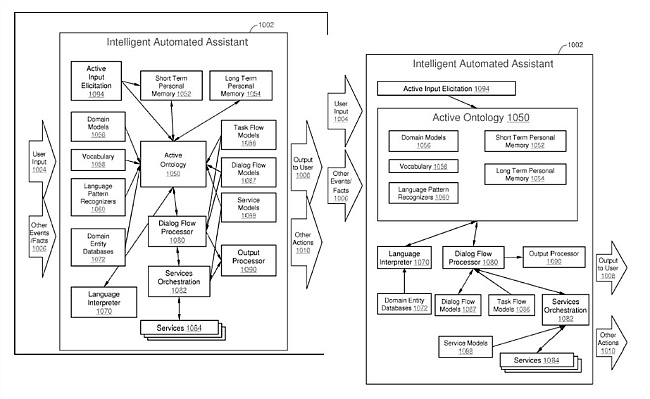
\includegraphics[scale=0.3]{Active_Ontology.jpg}
%				
%					Abbildung: Siris Komponenten \cite{imagesSiri}
%					
%				\end{column}
%				\hfill
%				\begin{column}{0.4\textwidth}
%					
%					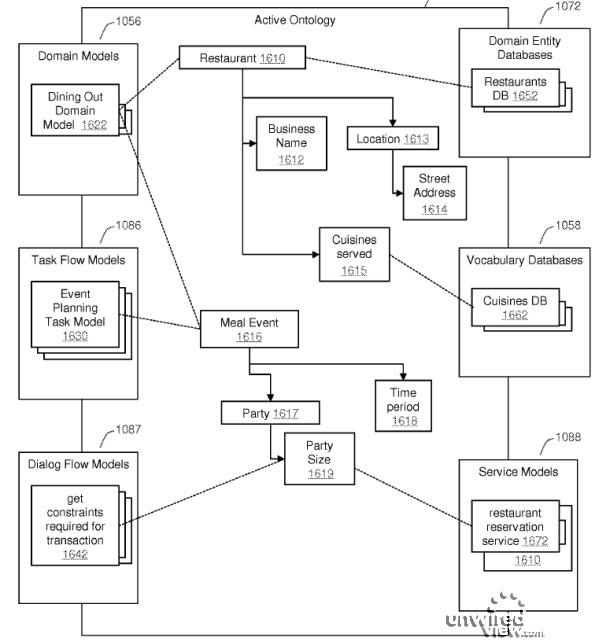
\includegraphics[scale=0.3]{Siri-iPhone-4S-iOS-active-ontology.jpg}
%					
%					Abbildung: Beispiel für die aktive Ontologie eines Restaurants \cite{imagesSiri}
%
%				\end{column}
%			\end{columns}
%			
%		\end{frame}
%
%
%	\subsection{Google Voice Search}
%	
%		\begin{frame}{Google Voice Search}
%
%			\begin{columns}[T]
%				\begin{column}{0.7\textwidth}
%					\begin{itemize}
%						\item Entstand als eine spezielle Suchfunktion der Google Inc.
%						\item Heute ist Google Voice Search im Google Now App integriert
%						\item für die Betriebssysteme Android und iOS verfügbar \newline \newline
%					\end{itemize}
%				\end{column}
%				\hfill
%				\begin{column}{0.3\textwidth}
%					
\includegraphics[scale=0.3]{GoogleLogo.png}
%				\end{column}
%			\end{columns}
%	
%			\begin{columns}[T]
%				\begin{column}{0.6\textwidth}
%					\begin{itemize}
%						\item Google Now wird durch den Google Assistant (s. Abbildung rechts) abgelöst
%					\end{itemize}
%				\end{column}
%				\hfill
%				\begin{column}{0.4\textwidth}
%					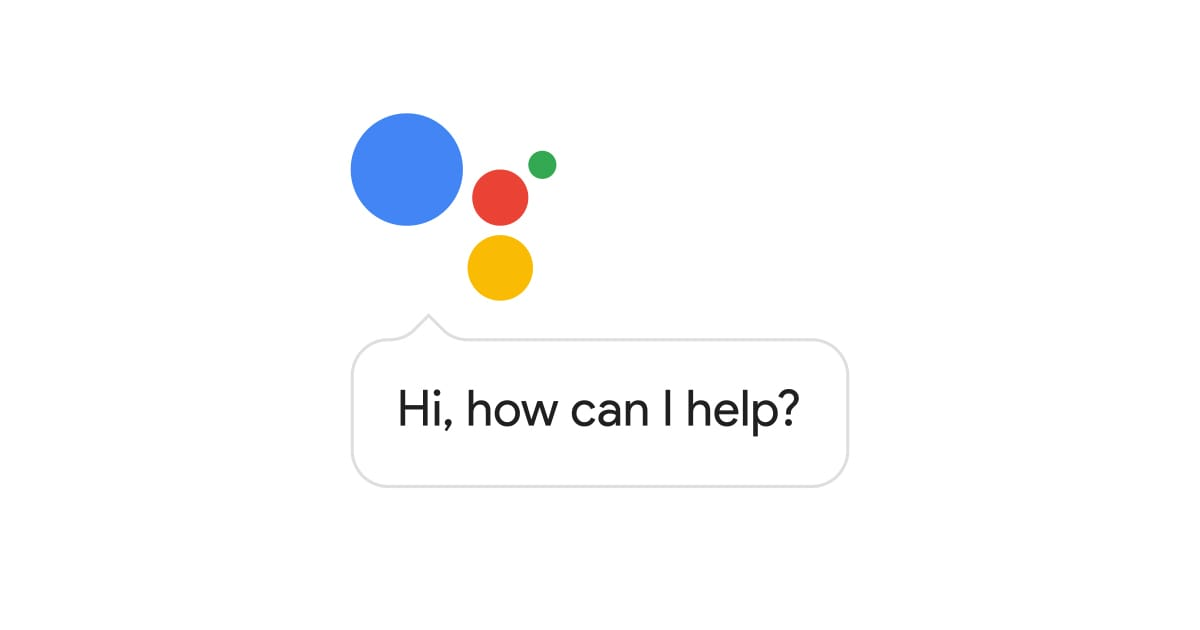
\includegraphics[scale=0.1]{googleassistant.jpg}
%				\end{column}
%			\end{columns}		
%		
%		\end{frame}
%	
%		\begin{frame}{Google Voice Search: Funktionen}
%			
%			\begin{block}{Aktivieren}
%				\begin{itemize}
%					\item ''Okay Google"
%				\end{itemize}
%			\end{block}
%			
%			\begin{exampleblock}{Unterstützte Funktionen}
%				\begin{itemize}
%					\item Begrenzte Offline-Aktionen wie Musik spielen lassen, Mail öffnen und WiFi aktivieren (Voice Action)
%					\item Internetsuche und gekoppelte Appfunktionen
%					\item Situationsbedingte Information
%					\item Semantische Suche
%				\end{itemize}
%			\end{exampleblock}
%			
%			\begin{alertblock}{Zusätzliche Funktionen}
%				\begin{itemize}
%					\item Google Now Empfehlungen in Form von "Karten"
%					\item Zusammenfassung des Bildschirminhalts mit "Now on Tap" 
%				\end{itemize}
%			\end{alertblock}
%			
%		\end{frame}
%	
%		\begin{frame}{Google Voice Search: Technologien}
%		
%			\begin{columns}[T]
%				\begin{column}{0.6\textwidth}
%					\begin{itemize}
%						\item Cloud-basierte Servicelieferung und Verwendung von vielen Ressourcen
%						\item Forschung und die Entwicklung der Software in Google erfolgt ''in vivo"
%						\item Googles Philosophie: "building models at scale"
%						\item Vorläufer von Google Voice Search - GOOG-411, Google Maps for Mobile und Google Mobile App
%						\item Entwicklung des User Interface in Verbindung mit dem Benutzerfeedback
%					\end{itemize}
%				\end{column}
%				\hfill
%				\begin{column}{0.4\textwidth}
%					\begin{figure}[h]
%						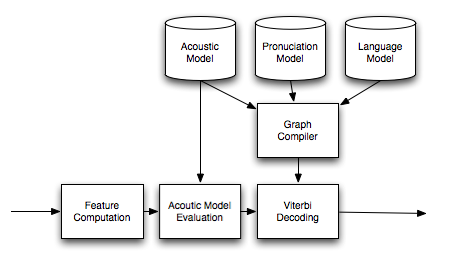
\includegraphics[scale=0.3]{SpeechRecognizer.png}
%						\centering
%						\caption{Blockdiagramm der Spracherkennungssoftware \cite{GoogleVoice}}
%						\label{fig:google1}
%					\end{figure}
%				\end{column}
%			\end{columns}
%		
%		\end{frame}
%
%	\subsection{Cortana}
%		
%		\begin{frame}{Cortana}
%			
%			\begin{columns}[T]
%				\begin{column}{0.7\textwidth}
%					\begin{itemize}
%						\item Software von Microsoft, ursprünglich für Windows Phone 8
%						\item Auf Windows 10, Android und iOS (Betaversion) verfügbar
%						\item In China unter dem Namen "Xiao Na" \newline \newline
%					\end{itemize}
%				\end{column}
%				\hfill
%				\begin{column}{0.3\textwidth}
%					
\includegraphics[scale=0.4]{CortanaLogo.jpg}
%				\end{column}
%			\end{columns}
%		
%			\begin{columns}[T]
%				\begin{column}{0.6\textwidth}
%					\begin{itemize}
%						\item Cortanas 18 Emotionen
%					\end{itemize}
%				\end{column}
%				\hfill
%				\begin{column}{0.4\textwidth}
%					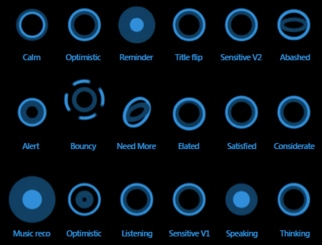
\includegraphics[scale=0.3]{cortana-emotions.jpg}
%				\end{column}
%			\end{columns}
%	
%			
%		\end{frame}
%	
%		\begin{frame}{Cortana: Funktionen}
%			
%			\begin{block}{Aktivieren}
%				\begin{itemize}
%					\item "Hey Cortana"
%				\end{itemize}
%			\end{block}
%			
%			\begin{exampleblock}{Unterstützte Funktionen}
%				\begin{itemize}
%					\item Offline-Aktionen, App-bedingte Suche und Bing-Recherche
%					\item Service für Erkennung von Liedern, Würfel rollen lassen, Münze werfen
%					\item Erinnerungen in Verbindung mit Kontakten
%					\item Nachrichtensynchronisation
%				\end{itemize}
%			\end{exampleblock}
%			
%			\begin{alertblock}{Zusätzliche Funktionen}
%				\begin{itemize}
%					\item Cortanas Notizbuch
%					\item Auf Events basierte Funktionen
%				\end{itemize}
%			\end{alertblock}
%			
%		\end{frame}
%	
%		\begin{frame}{Cortana: Technologien}
%			
%			\bigskip
%			
%			\begin{figure}[h]
%				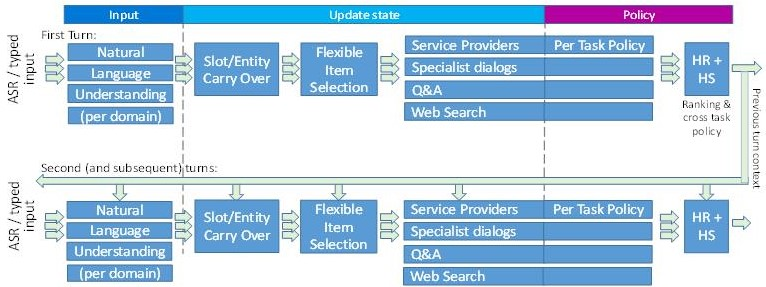
\includegraphics[scale=0.4]{cortana-architecture.png}
%				\centering
%				\caption{Cortanas Systemarchitektur \cite{cortanapaper}}
%				\label{fig:cortanasystem}
%			\end{figure}
%			
%			\begin{itemize}
%				\item Cortana Skills Kit
%			\end{itemize}
%			
%		\end{frame}

%\section{Vergleich und Bewertung der Assistenten}
%	\begin{frame}{Vergleich und Bewertung der Assistenten}
%		
%		\begin{block}{Funktionen}
%			\begin{itemize}
%				\item Googles Ökosystem (Play Music, Chromecast etc.)
%				\item Googles App-übergreifende Analyse
%				\item Lokale Offline-Spracherkennung bei Google Voice Search und Cortana
%				\item Cortanas originaler Funktionsumfang - Erkennung von Lieder, Würfel rollen lassen, Münze werfen und achtzehn Emotionen
%			\end{itemize}
%		\end{block}
%	
%	\end{frame}
%
%	\begin{frame}{Vergleich}
%		
%		\begin{block}{Technologien}
%			\begin{itemize}
%				\item Googles Wissensdatenbank „Knowledge-Graph“ und "Featured Snipets"
%				\item Google setzt sich mit der Anzahl und Genauigkeit der beantworteten Anfragen durch
%			\end{itemize}
%		\end{block}
%	
%		\begin{figure}[h]
%			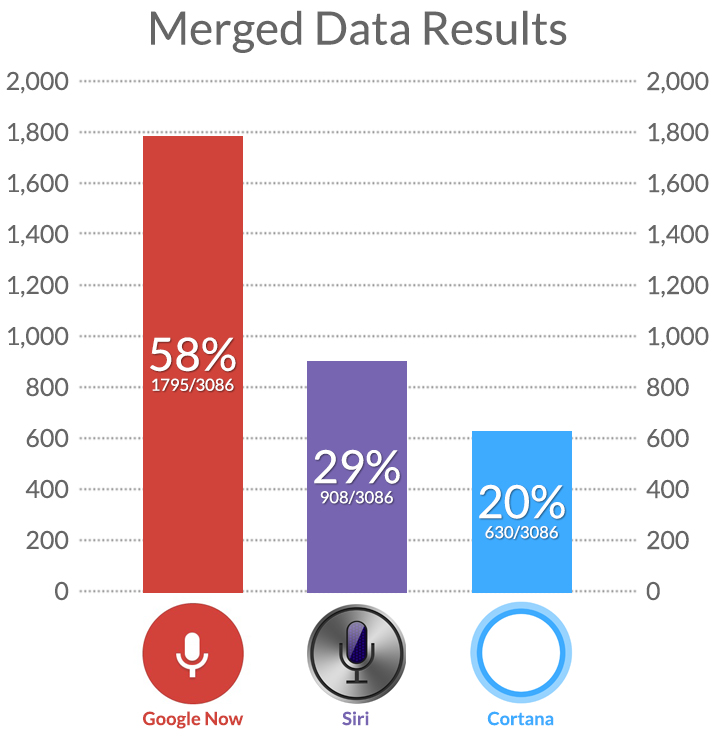
\includegraphics[scale=0.5]{vergleichStat.jpg}
%			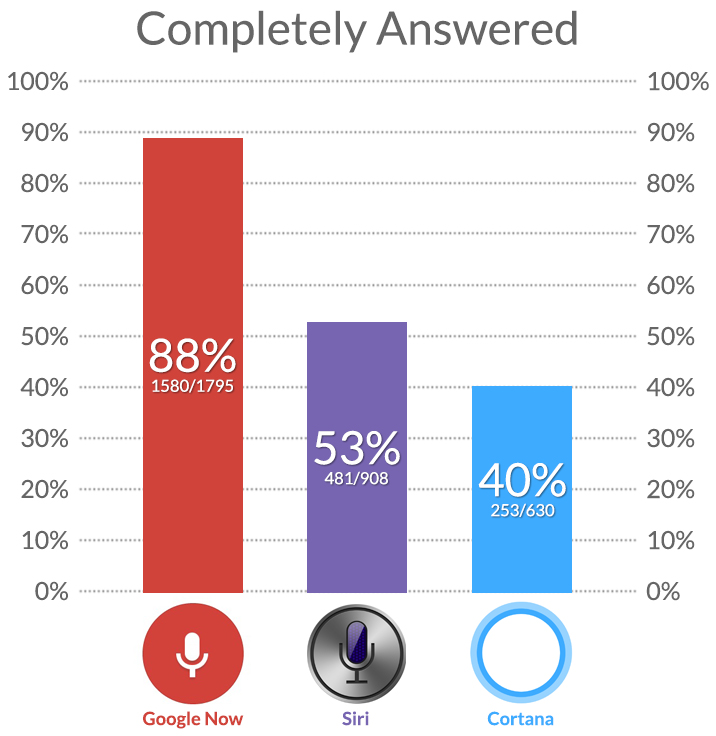
\includegraphics[scale=0.5]{vergleichStat2.jpg}
%			\centering
%			\caption{Ratio of returned results to asked questions (links), Ratio of returned results to correct results (rechts);  October 4, 2014. \cite{vergleichStat}}
%			\label{fig:vergleichImg}
%		\end{figure}
%	
%	\end{frame}
%	
%	\begin{frame}{Vergleich}
%	
%		\begin{block}{Betriebssysteme und Geräte}
%			\begin{itemize}
%				\item \textbf{Windows}: Cortana\\ \textbf{iOS}: Siri, Cortana und Google Voice Search\\ \textbf{Android}: Google Voice Search und Cortana
%				\item Google Voice Search unterstützt rund \textbf{40} Sprachen, Siri - \textbf{21} und Cortana \textbf{7}
%			\end{itemize}
%		\end{block}
%		
%		\begin{block}{User Experience}
%			\begin{itemize}
%				\item Siris und Cortanas lustige Persönlichkeiten\\ "Do you have a family?" \\
%				''I have you. That's enough family for me'' - Siri\\
%				''It is, for lack of a better word, impossible.'' - Cortana
%				\item Subjektive Einschätzung
%			\end{itemize}
%		\end{block}
%		
%	\end{frame}
%		
%	\begin{frame}{Vergleich}
%		
%		\begin{columns}[T]
%			\begin{column}{0.6\textwidth}
%				\begin{block}{Sicherheit}
%					\begin{itemize}
%						\item Funktionalität basiert auf ständiges Zuhören
%						\item Spekulation über Aufzeichnung und Auswertung der Umgebungsgeräusche
%						\item Cortanas Notizbuch ist eine Innovation 
%					\end{itemize}
%				\end{block}
%			\end{column}
%			\hfill
%			\begin{column}{0.4\textwidth}
%				\begin{figure}[h]
%					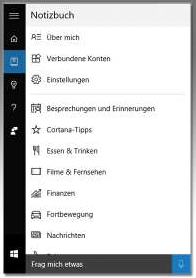
\includegraphics[scale=0.5]{CortanaNotebook.jpg}
%					\caption{Cortanas Notizbuch}
%				\end{figure}
%			\end{column}
%		\end{columns}
%	
%	\end{frame}
%
%\section{Zusammenfassung}
%	\begin{frame}{Zusammenfassung}
%	
%		\begin{exampleblock}{Schlussfolgerung}
%			\begin{itemize}
%				\item Google Voice Search gewinnt im Bereich der Spracherkennung, App-übergreifender Funktionalität und Marktdominanz
%				\item Cortana hat innovativen Charakter $\rightarrow$ Skills Kit
%			\end{itemize}
%		\end{exampleblock}
%	
%		\begin{itemize}
%			\item Ersatz bestimmter Dienstleistungen durch die digitalen Assistenten in naher Zukunft 
%			\item Die Assistenten laufen schon auf eigene Hausgeräten\newline
%		\end{itemize}
%
%		\begin{figure}[h]
%			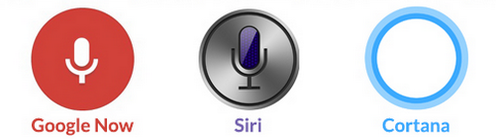
\includegraphics[scale=0.5]{SCG.png}
%		\end{figure}
%	
%	\end{frame}

\appendix

\begin{frame}[allowframebreaks]{Literatur}

%% --------------------
%% |   Bibliography   |
%% --------------------

\bibliographystyle{alphadin}	% german style

\section{Literatur}
\begin{thebibliography}{9}
	
	\bibitem{active} 
	Didier Guzzni, Adam Cheyer, Charles Baur. 
	\textit{Active, a platform for building intelligent software}. 
	IEEE Web Intelligence and Intelligent Agent Technology Workshops, 2006.
	
	\bibitem{dialog} 
	Alexander Wachtel, Jonas Klamroth, Walter F. Tichy. 
	\textit{A Natural Dialog System Based on Active Ontologies}.
	Annalen der Physik, 322(10):891–921, 1905.
	
	\bibitem{siriTech} 
	Steven Levy.
	\textit{An exclusive inside look at how artificial intelligence and machine learning work at Apple}.
	\\\texttt{https://www.wired.com/2016/08/an-exclusive-look-at-how-ai-and-machine-learning-work-at-apple/}
	
	\bibitem{siriPrivacy} 
	Informationen zum Sicherheitsinhalt von iOS 7.1.2.
	\\\texttt{https://support.apple.com/de-de/HT203014}
	
	\bibitem{tech} 
	Bernadette Johnson.
	\textit{How Siri Works}.
	\\\texttt{http://electronics.howstuffworks.com/gadgets/high-tech-gadgets/siri.htm}
	
	\bibitem{imagesSiri} 
	Stasys Bielinis.
	\textit{How Siri on iPhone 4S works and why it’s a big deal. Apple’s AI tech details in 230 pages of patent app}.
	\\\texttt{http://www.unwiredview.com/2011/10/12/how-siri-on-iphone-4s-works-and-why-it-a-big-deal-apple's-ai-tech-details-in-230-pages-of-patent-app/}
	
	\bibitem{GoogleVoice} 
	Johan Schalkwyk, Doug Beeferman, Francoise Beaufays, Bill Byrne, Ciprian Chelba, Mike Cohen, Maryam Garret, Brian Strope. 
	\textit{Google Search by Voice: A case study}. 
	
	%not used yet
	\bibitem{automatic} 
	Ciprian Chelba, Dan Bikel, Maria Shugrina, Patrick Nguyen, Shankar Kumar. 
	\textit{Large Scale Language Modeling in Automatic Speech Recognition}. 
	
	\bibitem{google} 
	Voice Search
	\\\texttt{https://www.xovi.de/wiki/Voice\_Search}
	
	\bibitem{googleAssistant} 
	Matthew Lynley.
	\textit{Google unveils Google Assistant, a virtual assistant that’s a big upgrade to Google Now}.
	\\\texttt{https://techcrunch.com/2016/05/18/google-unveils-google-assistant-a-big-upgrade-to-google-now/}
	
	\bibitem{googleChrome} 
	Get notifications from Google Now in Chrome 
	\\\texttt{https://chrome.googleblog.com/2014/02/get-notifications-from-google-now-in.html}
	
	\bibitem{googlenowontap} 
	Use Google Now on tap
	\\\texttt{https://support.google.com/websearch/answer/6304517?hl=de}
	
	\bibitem{googlelanguages} 
	Mariella Moon.
	\textit{Google Voice Search can now handle multiple languages with ease}.
	\\\texttt{https://www.engadget.com/2014/08/15/google-voice-search-multi-language-default/}
	
	\bibitem{googleoffline} 
	Eric Ravenscraft.
	\textit{Use Some Google Now Voice Commands Without an Internet Connection}.
	\\\texttt{http://lifehacker.com/use-some-google-now-voice-commands-without-an-internet-1733336980}
	
	\bibitem{googleassistant} 
	Meet your Google Assistant
	\\\texttt{https://assistant.google.com/}
	
	\bibitem{cortanaChina} 
	Joe Belfiore.
	\textit{Windows Phone 8.1 Update brings Cortana to new markets + new features}.
	\\\texttt{https://blogs.windows.com/windowsexperience/2014/07/30/windows-phone-8-1-update-brings-cortana-to-new-markets-new-features/JWs4xbDf9Di7x5Zu.97}
	
	\bibitem{cortanaAndroid} 
	Mary Jo Foley.
	\textit{Microsoft gears up for Cortana on Android preview}.
	\\\texttt{http://www.zdnet.com/article/microsoft-gears-up-for-cortana-on-android-preview/}
	
	\bibitem{cortanaReminders} 
	Brad Sams.
	\textit{Windows 10: Cortana now syncs reminders}.
	\\\texttt{https://www.neowin.net/news/windows-10-cortana-now-syncs-reminders}
	
	\bibitem{cortanaPredict} 
	Virginia Backaitis.
	\textit{Why Microsoft's Cortana is 14 for 14 Calling World Cup Matches}.
	\\\texttt{http://www.cmswire.com/cms/big-data/why-microsofts-cortana-is-14-for-14-calling-world-cup-matches-025853.php}
	
	\bibitem{cortanaFunc} 
	Tina Sieber.
	\textit{Here’s how to make the most of Cortana, the Windows 10 digital assistant}.
	\\\texttt{https://www.digitaltrends.com/computing/get-know-cortana-windows-10/}
	
	\bibitem{cortanaSync} 
	Brad Sams.
	\textit{Cortana Can Now Sync Notifications From Your Android Phone To Your Windows 10 PC}.
	\\\texttt{https://www.thurrott.com/windows/windows-10/67251/cortana-can-now-sync-notifications-android-phone-windows-10-pc}
	
	\bibitem{cortanaHandsfree} 
	Daniel Rubino.
	\textit{Hands on with 'Hey Cortana' and the Lumia 930 Denim update}
	\\\texttt{https://www.windowscentral.com/hands-on-hey-cortana-video}
	
	\bibitem{cortanaLanguages} 
	Cortana's regions and languages
	\\\texttt{https://support.microsoft.com/en-gb/instantanswers/557b5e0e-0eb0-44db-87d6-5e5db6f9c5b0/cortana-s-regions-and-languages}
	
	\bibitem{cortanapaper} 
	R. Sarikaya, P.A. Crook, A. Martin, M. Jeong, J.P. Robichaud, A. Celikyilmaz, Y.B. Kim, A. Rochette, O.Z. Khan, X. Liu, D. Boies, T. Anastasakos, Y. Feizollahi, N.Ramesh, H. Suzuki, R. Holenstein, E. Krawczyk, V. Radostev. 
	\textit{An overview of end-to-end language understanding and dialog management for personal digital assistants}.
	
	\bibitem{cortanafunc} 
	Chris Hoffman.
	\textit{15 Things You Can Do With Cortana on Windows 10}.
	\\\texttt{https://www.howtogeek.com/225458/15-things-you-can-do-with-cortana-on-windows-10/}
	
	\bibitem{cortanastory} 
	Tom Warren.
	\textit{1The story of Cortana, Micrsoft's Siri killer}.
	\\\texttt{https://www.theverge.com/2014/4/2/5570866/cortana-windows-phone-8-1-digital-assistant}
	
	\bibitem{cortanaapps} 
	Five Things You Didn't Know About Cortana, Microsoft’s Virtual Assistant
	\\\texttt{https://www.recode.net/2014/9/22/11631126/five-things-you-didnt-know-about-cortana-microsofts-virtual-assistant}
	
	\bibitem{cortanaemotions} 
	Melissa Riofrio.
	\textit{Cortana's UI now expresses 18 different emotions. Siri remains detached and aloof}
	\\\texttt{http://www.pcworld.com/article/2881902/cortanas-ui-now-expresses-18-different-emotions-siri-remains-detached-and-aloof.html}
	
	\bibitem{cortanaskills} 
	Microsoft takes aim at Alexa with Cortana Skills Kit
	\\\texttt{https://www.engadget.com/2017/05/10/stub-microsoft-takes-aim-at-alexa-with-cortana-skills-kit/}
	
	\bibitem{vergleichPakSafe} 
	Steve Dent.
	\textit{Die Digitalen Assistenten im Vergleich – Teil 2 unserer Miniserie}.
	\\\texttt{http://www.paksafe.de/blog/die-digitalen-assistenten-im-vergleich-teil-2-unserer-miniserie}
	
	\bibitem{vergleichFeatureSnipets} 
	Adrianne Jeffries
	\textit{Google’s featured snippets are worse than fake news}.
	\\\texttt{https://theoutline.com/post/1192/google-s-featured-snippets-are-worse-than-fake-news}
	
	\bibitem{vergleichOS} 
	Peter Stelzel-Morawietz.
	\textit{Was taugen Siri, Cortana und Google Now?}
	\\\texttt{https://www.pcwelt.de/ratgeber/Spracherkennung-Siri-Cortana-Google-Now-im-Ueberblick-9847719.html}
	
	\bibitem{vergleichStat} 
	Eric Enge
	\textit{The Great Knowledge Box Showdown: Google Now vs. Siri vs. Cortana}.
	\\\texttt{https://www.stonetemple.com/great-knowledge-box-showdown/VoiceStudyResults}
	
	\bibitem{vergleichSpeed} 
	Jason Parker.
	\textit{Google Search vs. Siri: Voice search speed test}.
	\\\texttt{https://www.cnet.com/news/google-search-vs-siri-voice-search-speed-test-video/}
	
	\bibitem{vergleichSiriGSR} 
	Mehdi Assefi, Guangchi Liu, Mike P. Wittie, Clemente Izurieta. 
	Department of Computer Science, Montana State University.
	\textit{An Experimental Evaluation of Apple Siri and Google Speech Recognition}.
	
	\bibitem{vergleichFunny} 
	Britta O'Boyle, Chris Hall.
	\textit{Siri vs Cortana: Which is the funniest assistant?}.
	\\\texttt{http://www.pocket-lint.com/news/136238-siri-vs-cortana-which-is-the-funniest-assistant} 
	
\end{thebibliography}
\end{frame}

\end{document}
